\documentclass[a4paper,11pt]{report}
\usepackage[T1]{fontenc}
\usepackage[utf8]{inputenc}
\usepackage{lmodern}
\usepackage[francais]{babel}
\usepackage{graphicx}
\usepackage{setspace}
\usepackage{float}
\usepackage{pdfpages} 

\title{Recette du projet : MonsterShip}
\author{Olivier \bsc{Boissard}, Kevin \bsc{Boulala},\\Maxime \bsc{Dubois}, Antoine \bsc{Lavier}}

\begin{document}

\maketitle
\setcounter{tocdepth}{1}
\tableofcontents

\chapter{Introduction}
  Dans ce rapport, nous allons faire la recette du projet MonsterShip commencé le 16 Décembre 2015. Nous verrons ce qui était prévu, ce qui a été implémenté et comment les fonctionnalités ont été implémenté. Suivi des fonctionnalités manquantes, les idées qui sont venues au cours du développement, et un bilan de ce que nous avons appris avec cette expérience.
  
\chapter{Contexte}
  Dans le cadre de nos études de Master 2 Informatique, nous avons eu pour mission dans le module de Programmation d'Applications Distribuées de travailler en groupe à l'élaboration d'un projet utilisant JavaEE avec le serveur d'application WildFly puis de le développer. L'objectif est de développer un jeu accesisible depuis un navigateur. Le cahier des charges que nous avons écrit pour l'occasion est disponible en annexe.

\chapter{Description de MosnterShip}
  MonsterShip est un space opera se déroulant dans la zone de Sagittarius A*, au centre de notre galaxie. Nous contrôlons un vaisseau où l'équipage est composé de monstres. Pour améliorer le vaisseau, nous utilisons comme ressource première l'équipage qui fusionne avec la structure du vaisseau. Mais il faut aussi un certain nombre de monstres par module pour qu'il fonctionne correctement.

\chapter{Le développement}
  \section{La structure du projet}
    \subsection{Organisation du projet}
      Voici l'arobrescence du projet MonsterShip :
      \begin{description}
        \item[MonsterShip] racine du projet
        \begin{description}
          \item[monstership-ear] archive pour déployer l'application
          \item[monstership-ejb] src/main/java/com/monstership/
          \begin{description}
            \item[data] définit l'accès aux données
            \item[model] définit la structure de données du projet
            \item[service] gère les fonctionnalités de l'application 
            \item[util] outillage
          \end{description}
          \item[monstership-web] l'application web
          \begin{itemize}
            \item src/main/java/com/monstership/
            \begin{description}
              \item[controller]
              \item[rest]
              \item[util] 
            \end{description}
            \item src/main/webapp/
            \begin{description}
              \item[resources] 
              \item[WEB-INF]
              \item[./] 
            \end{description}
          \end{itemize}
          
          
        \end{description}
      \end{description}
    \subsection{Les technologies utilisées}
  \section{Les fonctionnalités implémentées}
    \subsection{Connexion et inscription}
    \subsection{Visualisation de la carte et déplacements}
    \subsection{Récolte de monstres}
\chapter{La suite}
  \section{Les fonctionnalités déjà attendues}
  \section{D'autres idées}
\chapter{Conclusion}
\chapter{Annexes}
  \section{Cahier des charges}
    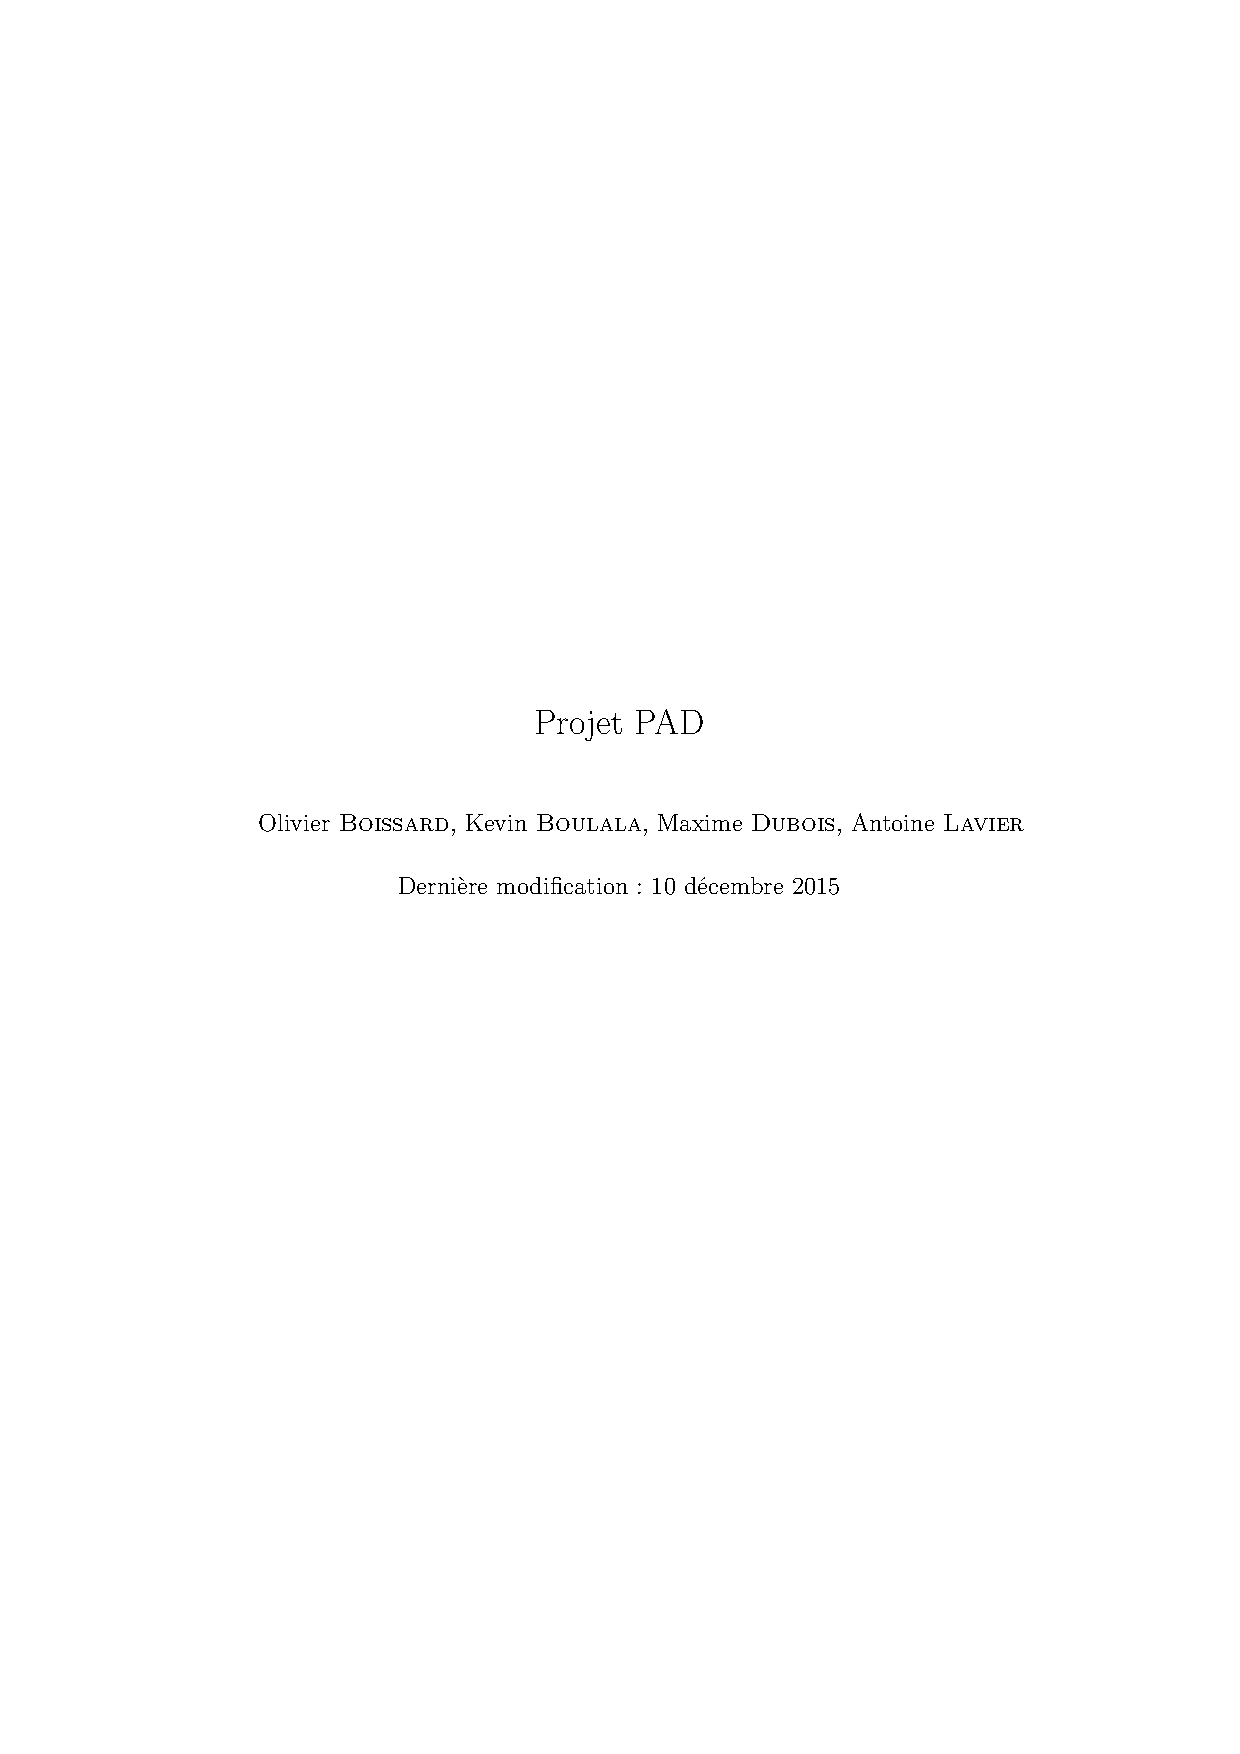
\includepdf[pages=1-17]{cahier_des_charges.pdf}
\end{document}
